\subsection{\label{MVC} Implementation of the \mvc}

The implementation of the \mvc provided by \pygtkmvc is a dialect 
version of the ``official'' pattern generally described by Software
Engineering Theory \footnote{For example, see
  \url{http://www.object-arts.com/EducationCentre/Overviews/MVC.htm}}.

\begin{figure}[htbp]
\begin{center}
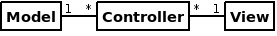
\includegraphics[width=6cm]{figs/png/mvc.png}
\caption{\label{MVC_f}Simplified Model-View-Controller Pattern}
\end{center}
\end{figure}
The implementation is different as the view side cannot see the model
part. The reasons behind this difference will be explained later, but
we can anticipate here that this is due to the relationship between
the view and the controller, that is stronger in \pygtkmvc than in the
classic \mvc. To a certin extend, in \pygtkmvc the view and the
controller parts are separate but could be considered as a unique
entity. However, a view can have multiple controllers (or a single
controller decomposed into many sub-controllers for the sake of
semplicity).

\smallskip

Figure \ref{MVC_f} shows three interconnected parts:

\begin{description}
\item[Model] Contains the \emph{state} (the \emph{logic}) of the
  application. Also it provides support to access and modify the
  state, and knows how to handle dependencies between different parts
  in the state. For example the application logic could require that
  changing a variable, causes a changing of another. It is not
  required the model user to be aware about this dependency, because
  model autonomously handles it.

  Zero, one or more \emph{Controllers} can be connected to one Model
  (see \emph{Controller}, below). Furthermore, one or more
  \emph{Views} can be associated with parts of the state; for example
  a numerical variable could be visualized as a number, as well as a
  graphic bar. It is important to remark that \emph{a Model does not
    know that a set of Views is possibly connected to its state
    through a set of Controllers}.

\item[View] shows parts of the Model state, and interactively
  exchanges information with the User, via input/output devices.
  A view can be dcomposed into sub-views to simplify the design and
  the reuse. 
  A View collects a set of widget trees built from a
  \glade file, and/or constructed by hand. Since a Widget contains a
  \emph{state}, this implementation differs from the standard \mvc,
  where generally the View side is completely \emph{stateless}.

  The View also interacts with zero, one or more \emph{Controllers}
  (see below), sending to it signals, and receiving information to
  visualize.

  A View does not know the semantics concerning what it visualizes,
  and neither knows that it is possibly connected to a set of
  controllers.

\item[Controller] Realizes the connection between Models and Views.
  A Controller contains the \gui logic: for example, it stores the
  information about what happens when a button is clicked (e.g. 
  handlers of signal are located inside a Controller.)

  A Controller perfectly knows the interfaces of the connected Model
  and View, and knows both the state and presentation (\gui)
  semantics. A Controller is associated to one Model (\emph{use a}
  relationship), and in the current implementation is associated
  only to one View (\emph{has a} relationship). A Controller may 
  grow in size, thus it is important to avoid including into the
  Controller code and information that should resize into the
  Model. Also Controller can be simplified by decomposing them into
  sub-controllers, each controlling a subset of the View. 

\end{description}

Two particular mechanisms make the isolation between Model and
Controller, and between View and Controller. To support the former,
the \obs is provided (see \ref{OBS}), whereas latter mechanism is
provided by the \mvc, and that is explained in \ref{VR}.


\subsubsection{\label{VR} View Registration}
Current implementation allows a N-1 relationship between Controller
and View. More clearly, one view can have multiple controllers
associated to it, meaning that a View can be shared among several
Controllers. A typical design for large views and controllers makes a
View be split into sets (not necessarily partitions) and each set is
controller by a sub-controller.

After a model and a view have been instantiated (model and view are
\emph{independent}, a controller can be constructed by passing them. 

From there on, the Controller can access the model, and teh view state
(the set of contained widgets). When the view registers itself with a
Controller, all signals are also automatically connected to the
corresponding methods inside the Controller.  Connection in this case
is performed by means of an implicit syntax rule, which binds a signal
name to a corresponding method name.

In sections \ref{VR:D} and \ref{VR:EX} more details and an example are
presented, to show how the View registration mechanism can be
exploited by controllers to connect signals and handle the creation of
particular widgets like for example TreeViews, TreeColumns,
CellRenderers, etc.
